\documentclass[a4paper]{article}

%% Sets page size and margins
\usepackage{fullpage}
\usepackage{geometry}

\usepackage[table]{xcolor} % Must come before packages that load xcolor

\usepackage{amsfonts}
\usepackage{amsmath}
\usepackage{amssymb}
\usepackage{array}
\usepackage{booktabs}
\usepackage{color}
\usepackage{enumerate}
\usepackage{graphicx}
\usepackage{mdwlist}
\usepackage{multicol}
\usepackage[all]{xy}
\usepackage{extarrows}
\usepackage[colorlinks=true, allcolors=blue]{hyperref}

\usepackage[normalem]{ulem}
\setlength{\parskip}{1ex}

\newcommand{\la}{\langle}
\newcommand{\ra}{\rangle}
\newcommand{\lra}{\longrightarrow}
\newcommand{\xlra}{\xlongrightarrow}
\newcommand{\tb}{\text{\textbullet}}
\newcommand{\sgn}{\text{sgn}}
\newcommand{\Tr}{\text{Tr}}
\newcommand{\im}{\text{im}}
\newcommand{\ol}{\overline}

\begin{document}

\title{Fixed Point Theorems and Evasiveness}
\author{Christopher Sumnicht}
\maketitle

\section{Introduction}

In the previous paper, we have concluded that for any simplex associated with a graph property to be nonevasive it must be collapsible. It may still be the case that there is an evasive property which is also collapsible. We can ask the question: Are there any graph properties which are not collapsible? This is still very much an active field of research, we will focus on one theorem in particular in this paper:

\begin{quote}
    Any nontrivial monotone graph property on a graph with a prime power of vertices is evasive.
\end{quote}

What is the general idea behind such a proof? Show that the associated simplicial complex is not collapsible!


\section{Collapsibilty and Being Acyclic}

Let's elaborate some more on the idea of collapsibility and smushing. Recall that we can collapse a complete triangle but not an empty triangle. We will impose some (admittedly bizzare) physical intuition for such a phenomenon.

Suppose that an a simplicial complex is embedded in $\mathbb{R}^n$ matching the dimension of the simplex. So, the triangle for instance would be embedded in $\mathbb{R}^2$. Imagine the space that doesn't include the simplex as solid. Next imagine the space that is the simplex as some sort of compressible fluid. In the case of the filled triangle, one can imagine taking their hand and compressing the fluid of the triangle completely to a single point. In the case of the empty triangle, there is a "rock" on the inside of the triangle preventing you from compressing the fluid of the empty triangle any further.

More generally, one can imagine that a simplicial complex is collapsible if one can take they're hand and after a series of squishes the structure, there are no rocks in your hand.

There are a couple ways to prove this see \cite{easy} and \cite{lecs}. However, in any case, the proof is rather involved. Ultimately, being able to smush the complex down to a single point implies that the structure is connected and has no holes in it. We call such a simplicial complex \textbf{acyclic}. As every collapsible simplicial complex can be smushed to a single point, every collapsible simplicial complex is acyclic.

\section{Fixed Points}

Now that we have (admittedly, somewhat informally) described our surface as one connected component with no holes, we can begin to apply some topological machinery to the space. We now exam an extremely important tool in topology: fixed points.

\subsection{Brouwer Fixed Point theorem}

\begin{quote}
    \textbf{Theorem (Brouwer)} Any continuous function from some geometric realization of a simplicial complex $\Delta$ (which we will denote $\ol{\Delta}$) fixes some point. In otherwords, say $f : \ol{\Delta} \to \ol{\Delta}$, then there is some $\delta \in \ol{\Delta}$ such that:
    $$f(\delta) = \delta$$
\end{quote}

We will instead prove a special case of this theorem. Nevertheless, the same general idea can be used to prove this variant of Brouwer's theorem, however, it gets quite a bit messier.

\begin{quote}
    \textbf{Theorem (Brouwer Open Ball)} Any smooth function (continuous and differentiable) function $f$ from the closed (unit) disc to itself has a fixed point.
\end{quote}

\begin{figure}
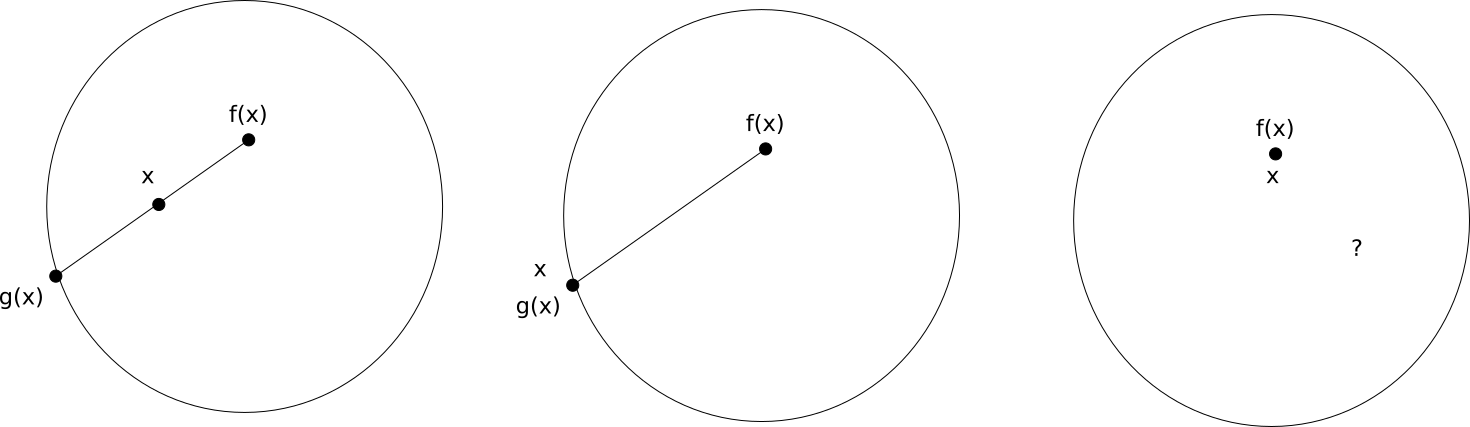
\includegraphics[height=4.5cm]{fixedpoint}
\centering
\caption{Possible different cases for $g(x)$, $x$ and $f(x)$. Left shows when $x$ is in the interior of the disc, the middle shows when $x$ is on the boundary, and the right is the case when $f(x) = x$ and the line segment is undefined.}
\end{figure}

\textbf{Proof} We make the following observation: 

\begin{quote}
    \textbf{Retraction Lemma} There is no smooth map $g : D \to \partial D$ such that $g \upharpoonright \partial D \to \partial D$ is equivalent to the identity on the boundary.
\end{quote}

It is often stated as: there is no way to retract the disc to it's boundary.

From this we will construct a function which is smooth but also the identity at the boundary given any smooth $f$ without fixed points.

As $f(x) \neq x$, we can construct a line from $f(x)$ through $x$ to the boundary. By calling this point $g(x)$ we get a new function $g : D \to \partial D$. Now, one important thing to to note is \textit{if} $f$ did indeed have a fixed point, it would be impossible to construct the ray! Now suppose that $x \in \partial D$, then $g(x) = x$ and so $g \upharpoonright \partial D$ is indeed the identity.

All we need to do now is show that $g$ is indeed a smooth function. As they $g(x)$, $f(x)$ and $x$ are all on the same line segment, it follows that:

$$g(x) = tx - (1 - t)f(x)$$

for some $t$. All we need to show is that $t(x)$ is a smooth function. This can be done by observing that $|g(x)| = 1$ so:

$$t^2|x - f(x)|^2 + 2tf(x)[x - f(x)] + f(x)^2 - 1 = 0$$

The solution to the equation can be obtained from the quadratic formula (or WolframAlpha), but the actual solution does not matter, really all that is necessary is to observe that the quadratic formula applied to smooth functions is again smooth and so it follows that $g$ is smoothe \textbf{Retraction Lemma} then implies that $g$ cannot exist. Contradiction.

\section{Abstract Simplicial Complex versus the Geometric Realization}

We make the following observation that there is a geometric realization of $f$. Call it $\ol{f}$. Observe that $\ol{f}$ is a continuous map from the geometric realization of $\Delta$ (we will refer to this as $\ol{\Delta}$ to the geometric realization of $\Delta'$ ($\ol{\Delta}$).

If $\ol{f}$ maps from $\ol{\Delta}$ to $\ol{\Delta}$, it follows that we can apply Brouwer Fixed Point theorem and notice that there is some fixed point $x \in \ol{\Delta}$ such that:

$$\ol{f}(x) = x$$

However, what $f$ does on the simplex is much more limiting than any arbitrary conitinuous function so we can get an even greater set of fixed points!

\begin{figure}
    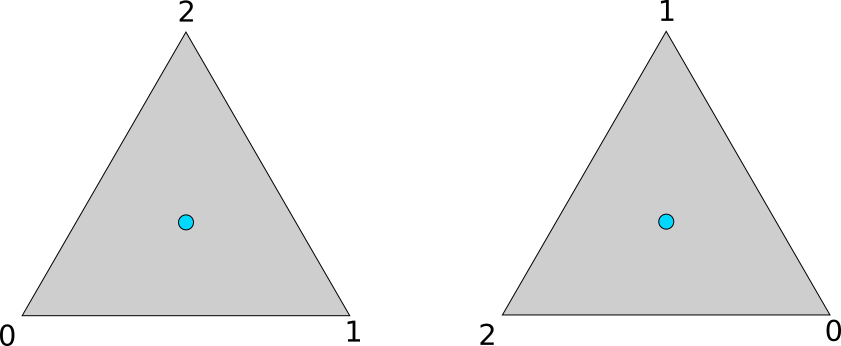
\includegraphics[height=4.5cm]{rotate}
    \centering
    \caption{The center of gravity is a fixed point of spinning a simplex.}
\end{figure}

\begin{quote}
    If $x \in \ol{\Delta}$ then $x$ is the sum of some linear combination of basis vectors. Define the \textbf{support simplex of $x$} $\Delta_x$ to be the collection of non-zero support vectors.
\end{quote}

Because of the way $f$ acts on a simplicial complex, for any the support of any fixed point:

$$f(\Delta_{x}) = \Delta_x$$

This intuitively says:

\begin{quote}
    If $x$ is a fixed point, then the face containing $x$ is fixed by the permutation.
\end{quote}

Furthermore, suppose $\ol{f}$ has some face. Then it may be the case the face was "rotated" from the original $\ol{\Delta}$, however it should be intuitive that this rotation does not affect the center point and so the center point is a fixed point for $f$.

\subsection{Orbits}

The rotations of these faces correspond to the "orbits" of $f$. Observing this fact we can almost conclude the following:

\begin{quote}
    If $P$ is a non-evasive monotone property that invariant under cycles it must be evasive.
\end{quote}

\textbf{Proof}: Suppose otherwise, then $P$ is non-evasive $\implies P$ is collapsible $\implies$ for any function $f$, $f$ has a fixed point. But the orbit of such a function must be $\{1, 2, 3, \ldots |V| \}$, the largest face of the graph which means that the completely connected graph does not satisfy the property.

\subsection{Finding the missing cycle}

We are almost ready to prove the main result. What we will plan to do now is show that there is a point that is fixed by every simplicial automophism.

\begin{quote}
    Let $\Gamma$ be a group of mappings and let $\Gamma'$ be a normal subgroup of order $p^k$ where $p$ is a prime. Suppose that $\Gamma/\Gamma'$ is cyclic, then every memeber of $\Gamma$ shares a fixed point.
\end{quote}

We will not go through a formal proof of this, but to gain an intuition for this when ever $x$ is a fixed point for $\Gamma$ we can "change the basis" representation of $x$ to be written in terms of any other permutation.

\section{Proof of Theorem}

From this we can finally conclude the result that we want:

\begin{quote}
    Every non-trivial monotone increasing property over a prime power of vertices is evasive.
\end{quote}

\textbf{Proof} Set $\Gamma$ to be the group of affine transformations (transformations of the form $ax + b$) and $\Gamma'$ to be the subgroup of translations (transformations of the form$x + b$). As $a$ and $b$ are in $\mathbb{Z}_{p^k}$, $\Gamma/\Gamma' \cong ax)$ which is cyclic. We leave it as an exercise to show that it is $\Gamma'$ is normal. But the orbits of these functions are $\{ 1, 2, 3, \ldots |V| \}$. Thus by the preceeding theorem, the connected graph must not satisfy the property and the property must be evasive.

\begin{thebibliography}{10}
\bibitem{orig}
Kahn, J., Saks, M. and Sturtevant, D. \textbf{A topological approach to evasiveness}. Combinatorica (1984) 4: 297. doi:10.1007/BF02579140

\bibitem{easy}
Miller, C. \textbf{ Evasiveness of Graph Properties and Topological Fixed-Point Theorems}. \url{https://arxiv.org/abs/1306.0110}

\bibitem{kleit}
Kleitman J. and Kwiatkowski J. \textbf{Further results on the Aanderaa-Rosenberg Conjecture}. (1980)

\bibitem{lecs}
Lovász, L. and Young N. \textbf{Lecture Notes on Evasiveness of Graph Properties}. (2002)

\bibitem{guil}
Guillemin V. and Pollack A. \textbf{Differential Topology}. (1974)

\end{thebibliography}

\end{document}
